% \documentclass[t, 10pt]{beamer}
\documentclass[t,handout, 10pt]{beamer}

\usepackage{graphicx}
\usepackage{epsfig}
\usepackage{psfrag}
\usepackage[english]{babel}
\usepackage{color}
%Mathematics packages
\usepackage{amsmath}
\usepackage{mathrsfs}
\usepackage{amsfonts}

\usepackage{enumerate}


\graphicspath{{./images/}} % Figures path - used in graphicx

\selectcolormodel{cmyk}

\mode<presentation>

%THEMES - Please refer to these chapters in the beamer documentation.
% Presentation themes : Chapter 15
% Color themes : Chapter 17
% Font themes : Chapter 18

\usetheme{Pittsburgh}
\usecolortheme{orchid}
\usefonttheme{default}

%---------------------------Title frame definition------------------------------------- 

\title{Usage Management In Multi-level Security Environments}
\author [Greg, Chris]{Gregory Heileman and Christopher C. Lamb}
\institute[University of New Mexico]{
\inst {}Department of Electrical and Computer Engineering\\
University of New Mexico}
\date{April 4, 2012}
\titlegraphic{
\begin{figure} 

\includegraphics[width = 10cm]{ECE-UNM-logo}
\end{figure}}

\begin{document}

\begin{frame}
\titlepage
\end{frame}

% This command will make the logo appear on all frames excluding the title frame.
\logo {
\includegraphics[width = 2.5cm]{UNM}}

\begin{frame}
\frametitle{Introduction}
\tableofcontents 
\end{frame}

\section{Information-centric Networking}
\begin{frame}
\frametitle{Information-centric Networking}

Information-centric networking (ICN) is a new approach to internet-scale networks.  These networks take advantage of data locality, cache data aggressively, decouple information providers from consumers, and use a content-centric perspective in network design
\pause
\newline
\newline
Similar conceptual approaches:
{\small
\begin{itemize}
\item {\bf Named Data Objects} --- Data objects are the primary data abstraction.
\item {\bf API Structure} --- Programming interfaces are structured around requesting specific data objects.  Can be synchronous or asynchronous.
\item {\bf Naming and Security} --- Names are tightly and securely bound to content.
\item {\bf Caching} --- Content is aggressively cached on nodes.
\end{itemize}
}
\pause
We are most concerned with the first and second characteristics currently.
\end{frame}

\begin{frame}
\frametitle{Current Technology Fail}
Current internet technologies don't dynamically protect data.  Initial design assumtions and implementation characteristics make these approaches difficult.
\pause
\newline
\newline
Why does the internet fail?
{\small
\begin{itemize}
\item {\bf Strict Layering} --- Routing and switching are generally lower level operations (layers 2 and 3 in the OSI model).  Content-sensitive routing is a layer 7 (application layer) operation, requiring very expensive hardware to do well. 
\item {\bf End-to-End Arguments} --- Network cores are simple, fast, and dumb.  They need to brighten up to evanluate information suitability.  
\item {\bf Packetization} --- Policies and content requires multiple packets.  This implies complex window retention logic to handle context splitting, and in at least half of typical cases, context splitting can't be handled at all.
\end{itemize}
}
The principles have been effective, but in some cases services {\it should} be in the network core.
\end{frame}

\section{System Overview}
\begin{frame}
\frametitle{System Overview --- Device Perspective}
\centerline{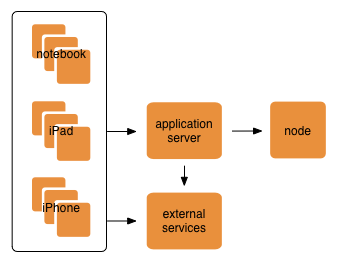
\includegraphics[width=2in]{overall-view}}
How does the system work?
\pause
{\small
\begin{enumerate}
\item {\bf Request} --- An initial request is submitted from an edge device
\pause
\item {\bf Reciept} --- The request is received by an application server that has access to ICN services via an ICN node and external services of some kind as well.
\pause
\item {\bf Dispatch} --- The request for information if suitable is dispatched into the ICN.
\end{enumerate}
}
\end{frame}

\begin{frame}
\frametitle{System Overview --- Into the network}
\centerline{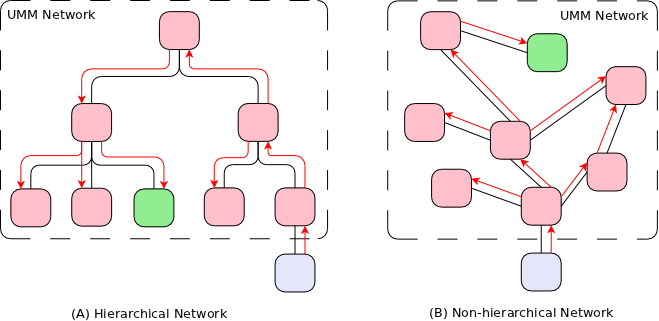
\includegraphics[width=3.5in]{node-hierarchy}}
How is information dispatched through the network? {\it Well, it depends on the network.}
\pause
{\small
\begin{enumerate}
\item {\bf Submission} --- Submit to a node.
\item {\bf Transmission} --- Pass through the network, either via a router (if hierarchical) or known peers (non-hierarchical).
\item {\bf Respond} --- Nodes respond with content if possible.
\end{enumerate}
}
\end{frame}

\begin{frame}
\frametitle{System Overivew --- Nodes and Routers}
\centerline{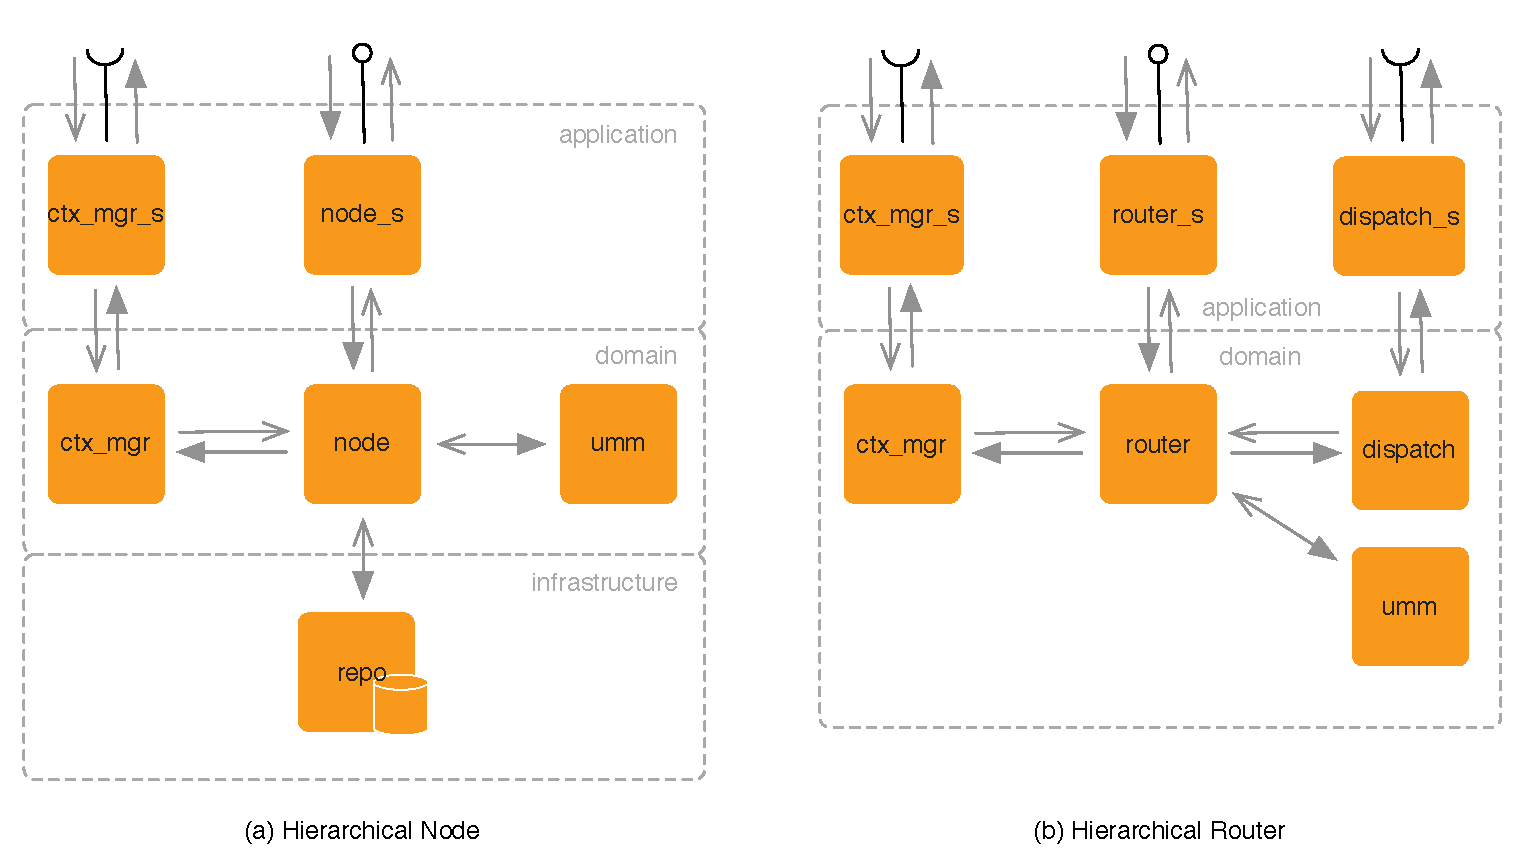
\includegraphics[width=3.5in]{router-node-view}}
\end{frame}

\section{Theoretical Foundations}
\begin{frame}
\frametitle{Distributed Security Decisions}
\end{frame}

\begin{frame}
\frametitle{Optimal Substructure}
\end{frame}

\begin{frame}
\frametitle{Overlapping Subproblems}
\end{frame}

\begin{frame}
\frametitle{Information Protection}
\end{frame}

\section{Implementation Overview}
\begin{frame}
\frametitle{Implementation Overview --- Simulation Environment}
\end{frame}

\begin{frame}
\frametitle{Implementation Overview --- Capistrano}
\end{frame}

\begin{frame}
\frametitle{Implementation Overview --- Rest API}
\end{frame}

\begin{frame}
\frametitle{Implementation Overview --- Information Flow}
\end{frame}

\begin{frame}
\frametitle{Implementation Overview --- Usage Domain}
\end{frame}

\begin{frame}
\frametitle{Implementation Overview --- Policy Language}
\end{frame}

\section{Final Steps}
\begin{frame}
\frametitle{Next Steps}
\end{frame}

\end{document}

